\textbf{\emph{Patient Data}}

We used the treatment information from 45 prostate, 10 breast, 10 lymph node, 10 head and neck and 10 liver patients who were previoulsy treated using the MRI-Linac Elekta Unity (Elekta, Stockholm, Sweden) in our institution. \textbf{List fieldsizes, and gantry angle distribution (maybe a fanfy plot with a circualr coordinate system, like a distribution over angles) respectively}. 
To to improve transational capabilities of the network 

List how many segments for which entity I used and then how i split them up into training, validation and test patients and their respective number of segments. to match CT image shape dose distribution were resized to match the 512x512x number of slices shape of the ct input array. (siehe workflow\_code/utils.py skripte). The original iso center of the plan was used weather it was centered in the volume or not. 

Ground truth dose distributions were calculated EGSnrc using 10\textsuperscript{7} histories. (information über EGSnrc also software version und release \cite{noauthor_nrc-cnrcegsnrc_2021}) Each segment was calculated using same number of monitor units which enabled me to scale the segment based on the segment weight when predicting an entire treatment plan. 

\textbf{\emph{Network}}

The U-Net expects a 3d input of size (batchsize, num\_masks, W, H, D) and samples this input over the encoding path down to extract important features on a lower level scale from size [W, H, D] down to [W/2, H/2, D/2]. The decoding is done using 3D transposed convolutions with a kernelsize and a stride of 2 respectively. A skip connecting was added to before pooling to pass on highler level of volume resolution to later parts of the U-Net. 
Each block building block consits of a convolutional layer with zero padding, to maintain dimensionality, kernel size 3x3x3 and a stride of 1, a 3D batch normalization layer and a RelU layer. No dropout was used. 
Modified version of (doi:10.1007/978-3-319-24574-4\_28)


\begin{figure}
	\centering
    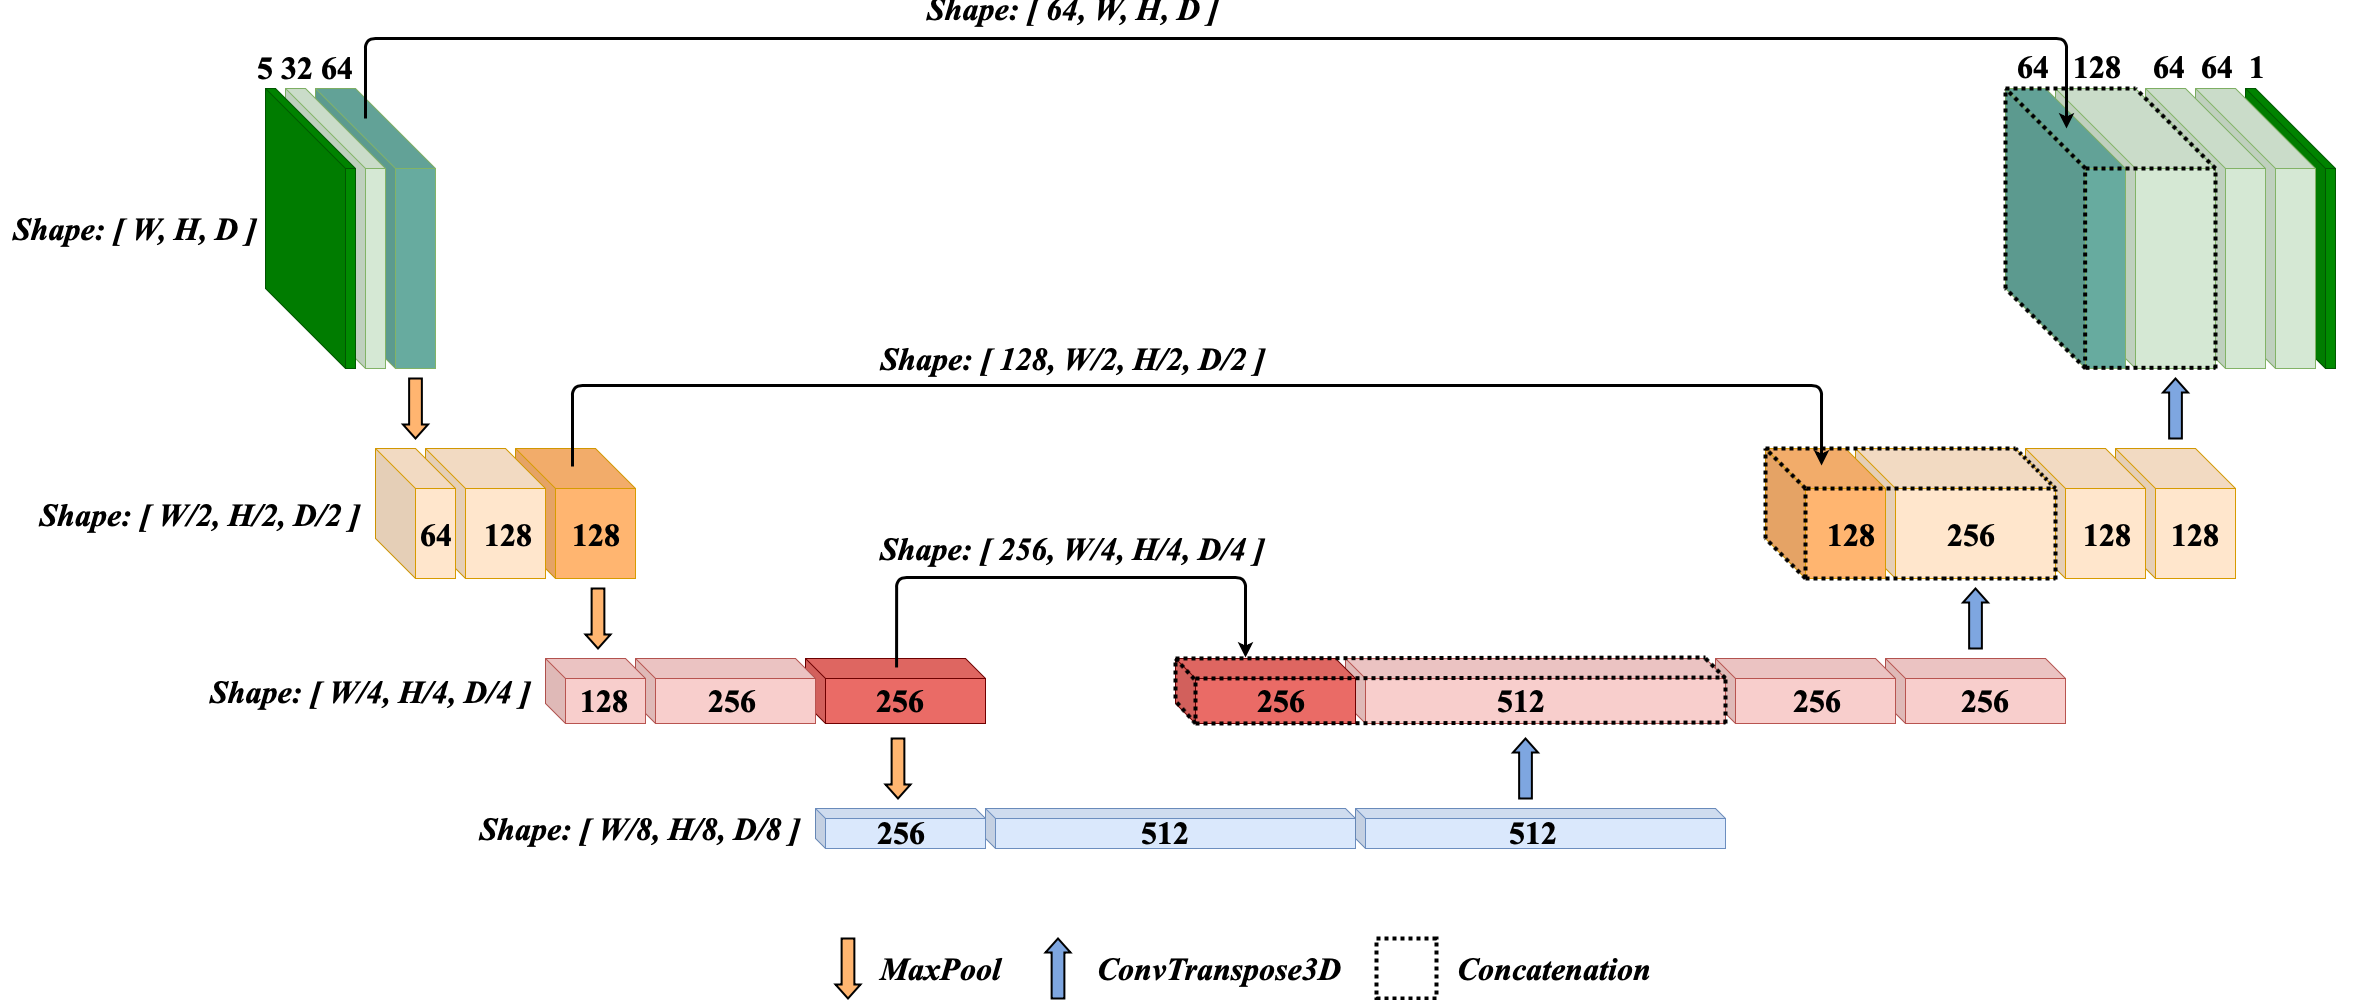
\includegraphics[width=\textwidth]{unet}
    \caption{3D U-Net architecture}
    \label{fig: unet}
\end{figure}

\textbf{\emph{Input Data}}

The input of the network consists of 5 different masks containig spatial information about the given volume. (insert image with different masks and a little description of it) refer to deepdose paper by kontaxis \cite{kontaxis_deepdose_2020}

\begin{figure}[H]
    \vspace{1cm}
    \minipage{0.32\textwidth}
        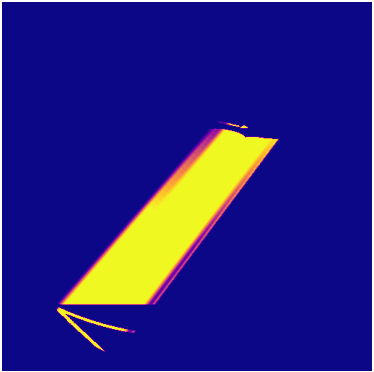
\includegraphics[width=4cm]{binary}
        \caption*{(a)}
    \endminipage\hfill
    \minipage{0.32\textwidth}
        \captionsetup{format=hang}
        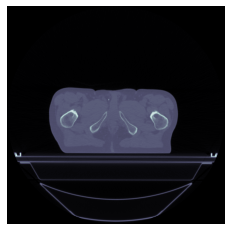
\includegraphics[width=4cm]{ct.png}
        \caption*{(b)}
    \endminipage\hfill
    \minipage{0.32\textwidth}%
        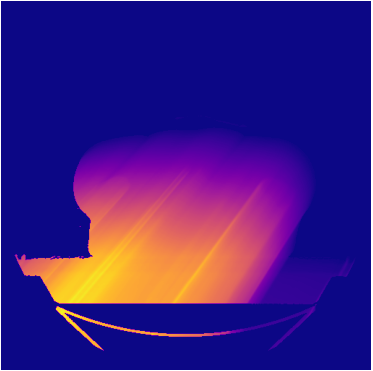
\includegraphics[width=4cm]{radio.png}
        \caption*{(c)}
    \endminipage
    \vspace{1cm}
    \minipage{0.49\textwidth}
        \centering
        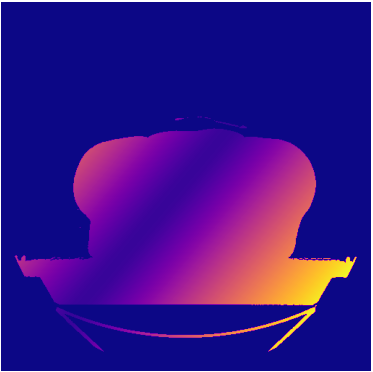
\includegraphics[width=4cm]{center}
        \caption*{(d)}
    \endminipage\hfill
    \minipage{0.49\textwidth}
        \centering
        
\includegraphics[width=4cm]{source}
        \caption*{(e)}
    \endminipage\hfill
    \caption{Input masks for training}\label{fig: masks}
\end{figure}

in the image above the the different input masks can bee seen. the masks are the binary beam shape (a), ct image with (electron density oder HU values, mal schauen was besser performed) (b) radiologial depth (c) center beamline distance (d) and source distance (d) 
the binary beam shape input is most importance, due to the fact that this input mask is the only one providing the network with information about the beam position and orientation concerning shape and limits

ct and readiological depth provide structural information about the parient anatomy. the radiological depth in particular helps the network to understand spatial dimensions when being given patches for training, becuase the information where a specific voxel is located inside the patients anatony would be lost when training with patches without the radiological depth. the algorithm for radiological depth calculation is implemented in python and based on  \cite{siddon_fast_1985}

all input masks are limited to the volume where the ct mask has a houndsfield unit value higher than 150, since this is the threshhold of our institunional dose esmiation software.

The entire network and training algorithm is programmed in PyTorch. The dataloading was inspired by TorchIO, a libary for efficient dataloading for 3d medical imaging and especially patch based loading of 3d data. (torch io citen \cite{perez-garcia_torchio_2021}) Due to the immense memory usage of (nummer an segmenten angeben) segments, not all segments could be loaded simutaneously into the memory. to archieve a randomised set of patches presented to the network at each training itteration, the dataloading is based on a subset of patient segments randomly selected from the entire training data pool. To further inprove dataloading time, a simutaneous loading of multiple segments at the same time using multi threading was implemented. 

\begin{figure}
    \centering
    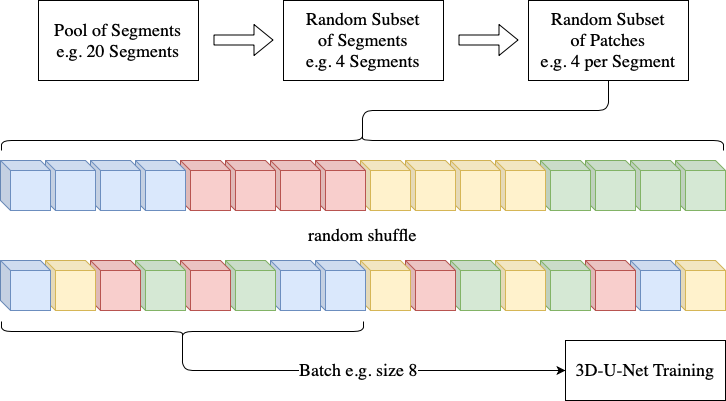
\includegraphics[width=.8\textwidth]{dataloading}
    \caption{Dataloading scheme}\label{fig: dataloading}
\end{figure}

(referenz auf bild was dataloading verdeutlicht) shows the schematic process of preloading a data queue from which random patches are taken for each batch presented the network for training. when the queue gets filled with patches a by the user specified number of segments gets randomly selected from the pool. then another by the user specified number of random patch positions per segment are extracted from the entire volume. then the entire queue gets shuffled and is then emptied during the training process. after the dataqueue is empty it is refilled with new patches from not previously used segments.
after all segments have been used for patch extraction, the list of available segments is reset.


\textbf{\emph{Training}}

The 3D-UNet was trained on a HPC cloud based solution using a 4 Nvidia GTX 2080 Ti with 11GB of VRAM. The batchsize for training was 128 and the patch size was 32 in all dimensions resulting in the input shape of (128, 5, 32, 32, 32). Since 4 graphics cards were used each card processed 32 patches of size (5, 32, 32, 32) simutaneously. The spatial resolution of a 32 x 32 x 32 patch was 37.4 x 37.4 x 96 mm\textsuperscript{3} with voxel dimensionality of 1.17 x 1.17 x 3 mm\textsuperscript{3}. 
The loss function used was the root mean squared error and the ADAM optimizer with a starting learning rate of 10\textsuperscript{-4}, and the standard settings for beta1, beta2 and epsilon of 0.9, 0.999 and 10-8 respectively. Learning rate was reduced by a factor of 10 when no improvement in the validation loss could be observed. 
A validation step was done after the training queue has been refilled resulting in a validation step after 12800 patches with 64 segments per queue and 200 patches per segment. The overall accuracy regarding the 3mm/3\% gamma values was assessed every 5 queue refillings. Training was stopped when no validation loss improvement could be observed for 30 epochs after learning rate reduction to 10\textsuperscript{-6}.

Training supervision was done using Tensorboard in which training loss, validation loss and a the gamma pass rate could be viewed during training. 


\textbf{\emph{Output analysis}}

To assess the overall performance of the network a gamma anlysis (cite gamma paper) was perfomed. The settings for individual segments and total plan are shown in Table \ref{tab: gamma_settings}.  

\begin{table}[]
    \captionsetup{singlelinecheck = false, format= hang, justification=raggedright, labelsep=space}
    \caption{Settings used for gamma analysis of single segments and entire radiation plans.}
    \label{tab: gamma_settings}
    \centering
    \begin{tabular}{@{}lcccc@{}}
        \multicolumn{1}{c}{} & \textbf{\begin{tabular}[c]{@{}c@{}}percentage \\ threshold\end{tabular}} & \textbf{\begin{tabular}[c]{@{}c@{}}distance \\ threshold\end{tabular}} & \textbf{\begin{tabular}[c]{@{}c@{}}lower \\ cutoff\end{tabular}} & \textbf{\begin{tabular}[c]{@{}c@{}}local \\ gamma\end{tabular}} \\
        \multicolumn{1}{c}{} & \textbf{/\%}                                                             & \textbf{/mm}                                                           & \textbf{/\%}                                                     & \textbf{/1}                                                     \\ \midrule
        segment              & 3 / 2 / 1                                                                & 3 / 2 / 1                                                              & 10                                                               & False                                                           \\
        plan                 & 3 / 2 / 1                                                                & 3 / 2 / 1                                                              & 40                                                               & False                                                           \\ \bottomrule
    \end{tabular}
\end{table}

Hier mal noch mit den anderen diskutieren, was man noch machen könnte. DVH? oder sonstige analysen der Dosis. z.B. diese Dice analyse die ich geplant hatte, wo man einen Threshold setzt und dann schauen wie sehr sich die prozente überschneiden.

\textbf{\emph{Testing}}

The model tested on only prostate patients was tested against all other entities so assess the translational capabilities of a model only trained on one entity. The model trained on prostate, liver, breast and head and neck radio treatment data, was evaluated on all entities trained on aswell as on lypmh nodes to asses the translation to a tumor entity which was not present in the training data. 






